\part{IHM}
\setcounter{section}{0}

\section{Enchainement des fenêtres - EDF}

\begin{figure}[H]
\noindent\makebox[\textwidth]{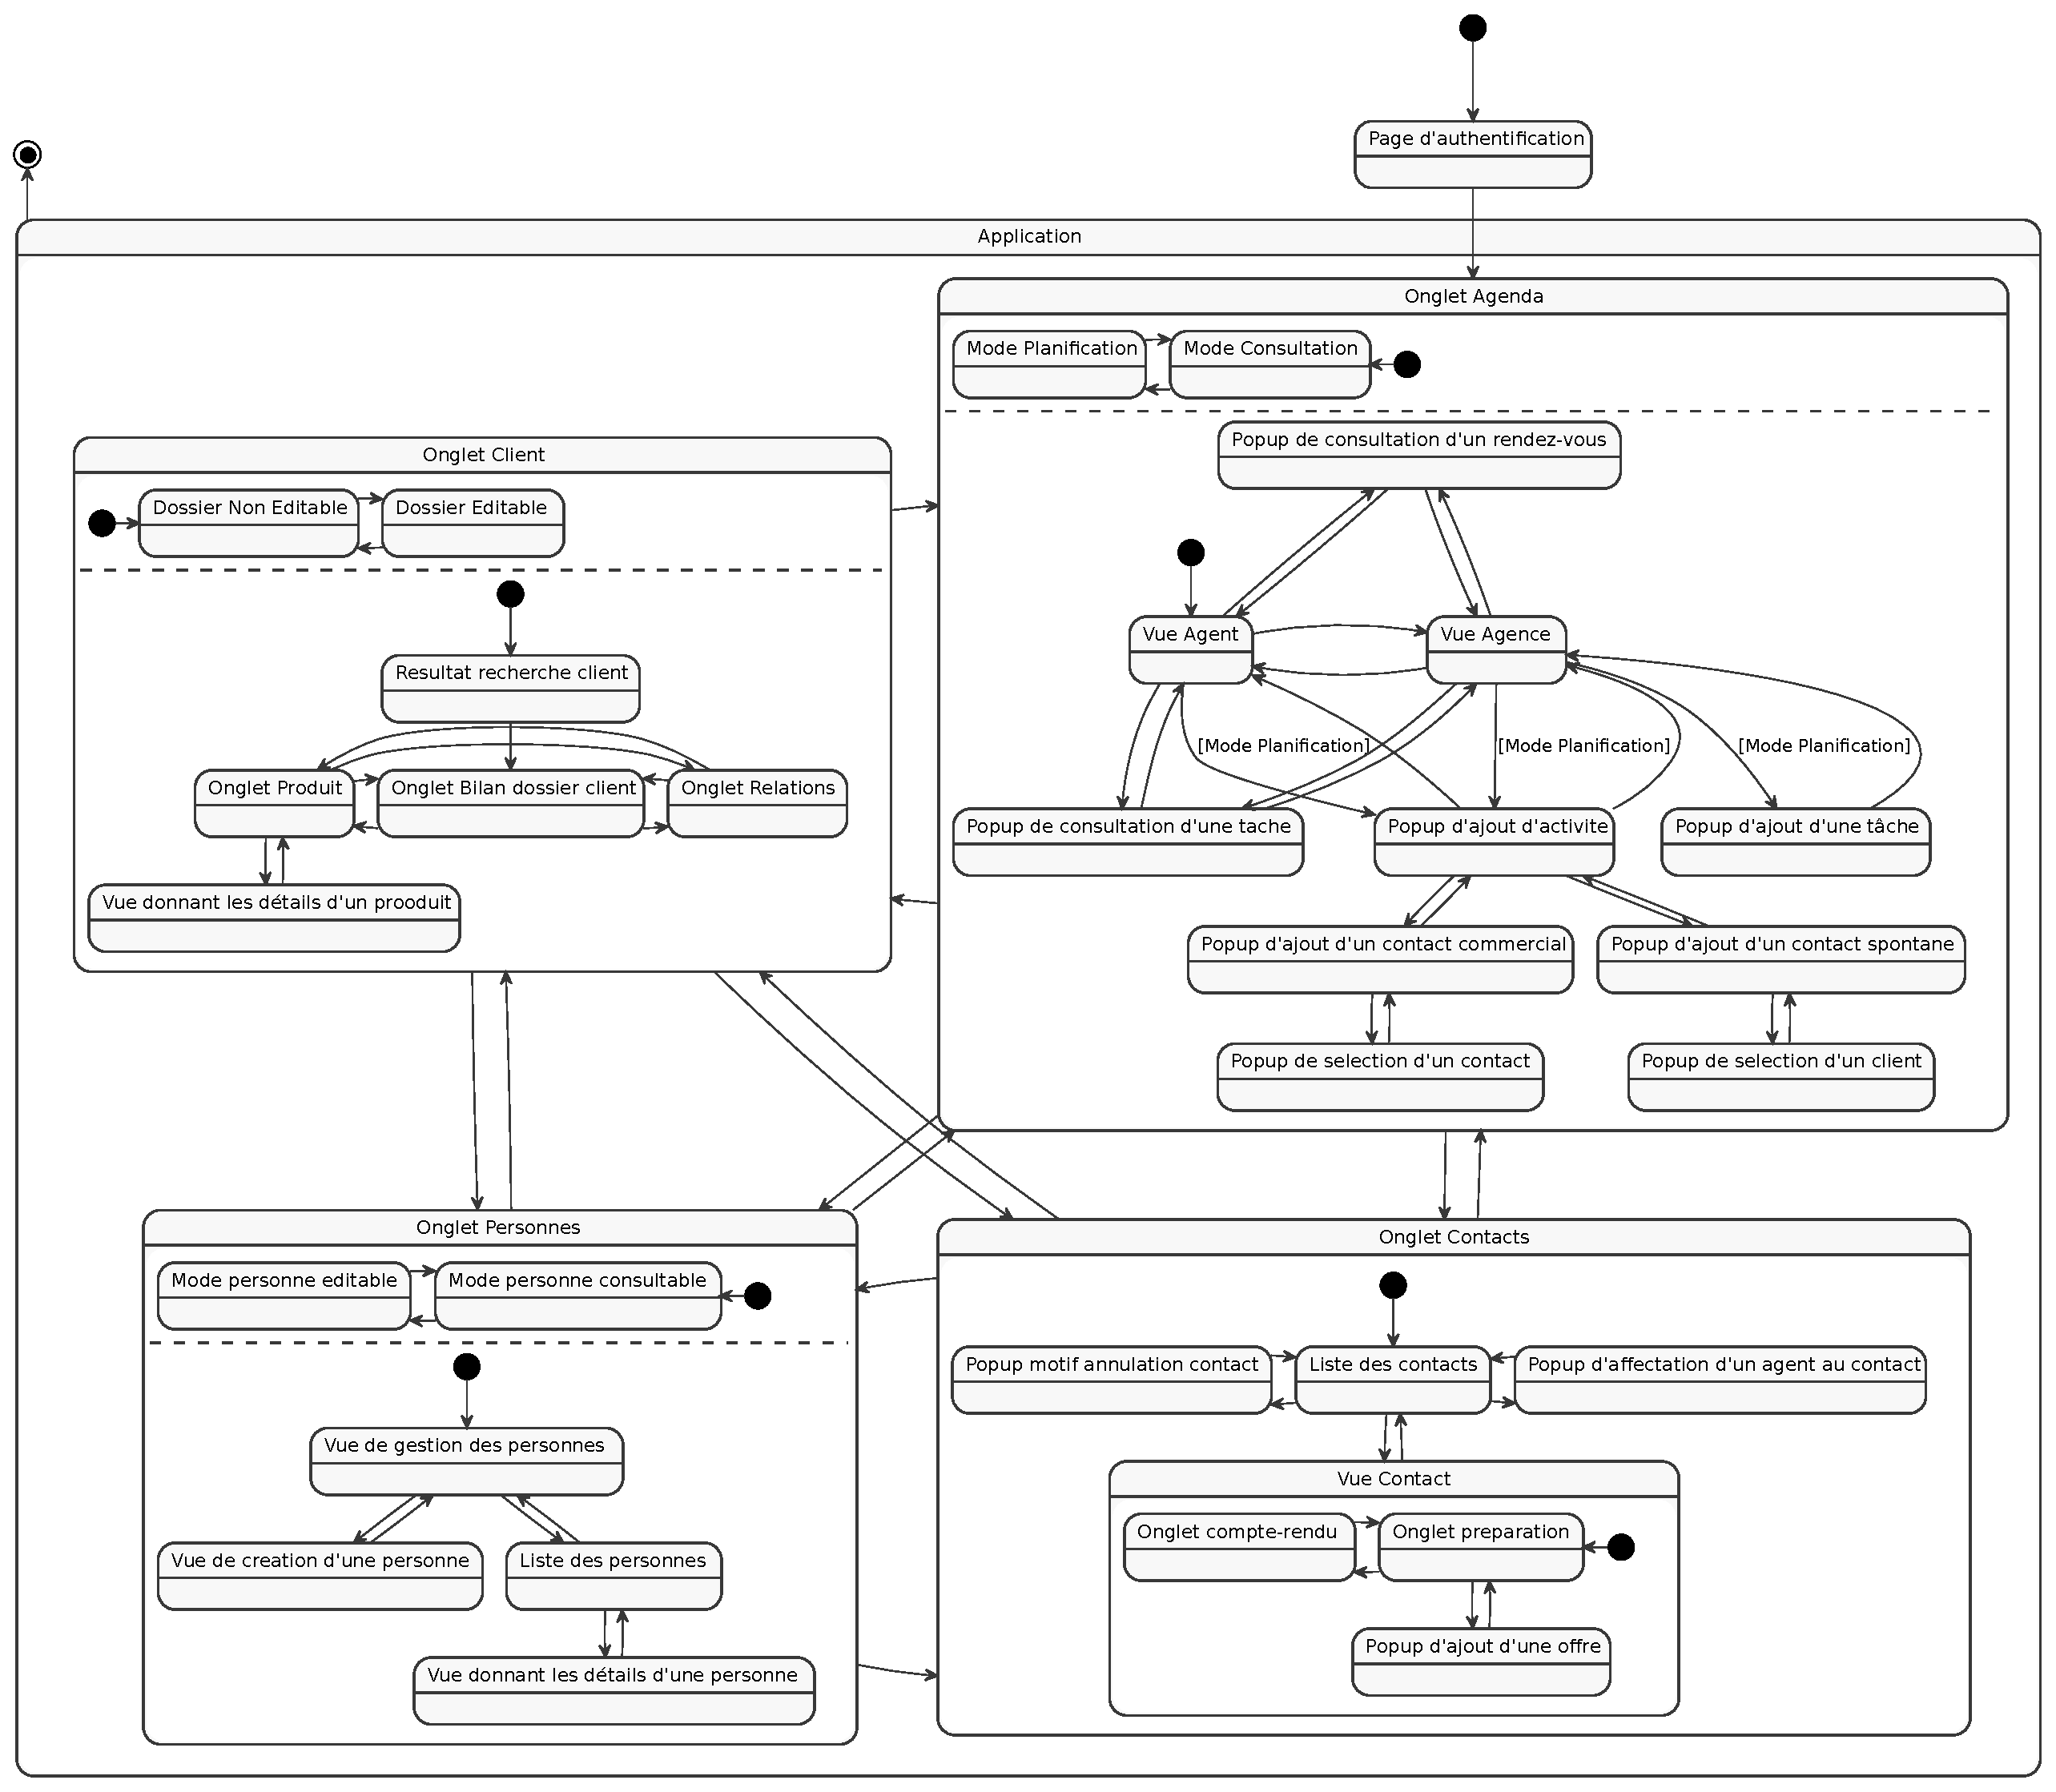
\includegraphics[width=18cm]{figures/eps/EdF}}
\caption{Diagramme d'enchainement des fenêtres}
\end{figure}

\section{Présentation des différentes vues}
Les vues de l'IHM sont présentées dans les pages suivantes.

\begin{shaded}
\textbf{Note: } Les tableaux récapitulant les SMA des différentes vues sont présentés par IHM. Si des services sont redondants, ils ont le même numéro et ne sont pas répétés dans le tableau. 
\end{shaded}

\includepdf[scale=0.8,angle=90,pages={2-9},pagecommand=\subsection*{IHM client}]{figures/IHM.pdf}


\begin{table}[H]
\centering
\caption{SMA - IHM Client}
\begin{tabular}{p{0.1\textwidth}p{0.4\textwidth}p{0.4\textwidth}}
\hline
Num & \multicolumn{1}{c}{Nom Contrôle} & \multicolumn{1}{c}{SMA} \\ \hline
\rowcolor[gray]{0.9}
\multicolumn{3}{l}{CU10 - Recherche des clients}  \\
1.1 & Bouton Rechercher & PAS DE SMA \\
\rowcolor[gray]{0.9}
\multicolumn{3}{l}{CU10 - Résultats recherche clients} \\ 
1.2 & Bouton Rechercher  & PAS DE SMA       \\             
1.3 & Bouton Voir le client & ObtenirClientEtAgence \newline ConsulterBilanClient \\
\rowcolor[gray]{0.9}
\multicolumn{3}{l}{CU10 - Bilan - Dossier Client}  \\
1.4 & bouton oeil  & ConsulterDetailPersonne \\
1.5 & bouton crayon  & ConsulterDetailPersonne \\
1.6 & bouton poubelle  & SupprimerPersonne \\
1.7 & onglet Produits  & ObtenirProduits \\
1.8 & onglet Relations  & ConsulterRelationsBanqueClient \\
\rowcolor[gray]{0.9}
\multicolumn{3}{l}{CU10 - Bilan - Dossier Client- Mode modification} \\ 
1.9 & Bouton Ajouter une personne  &  AjouterPersonne ou \newline CreerEtAjouterPersonne  \\             
1.10 & Bouton Enlever du client & SupprimerPersonne \\
1.11 & Bouton Valider & MAJEnteteDossier \\
\rowcolor[gray]{0.9}
\multicolumn{3}{l}{CU10 - Produits - Dossier client}  \\
1.12 & onglet Bilan & ConsulterBilanClient \\
1.13 & Bouton oeil & ConsulterDetailProduit \\
1.14 & Bouton Modifier (puis valider) & MAJComptesConcurrence \\
\rowcolor[gray]{0.9}
\multicolumn{3}{l}{CU10 - Détail produit - Dossier client} \\ 
\rowcolor[gray]{0.9}
\multicolumn{3}{l}{CU10 - Relations - Dossier client} \\ \hline
\end{tabular}
\end{table}


\includepdf[scale=0.8,angle=90,pages={10-14},pagecommand=\subsection*{IHM Personnes}]{figures/IHM.pdf}

\begin{table}[H]
\centering
\caption{SMA - IHM Personnes}
\begin{tabular}{ll}
\hline
\multicolumn{1}{c}{Num Contrôle} & \multicolumn{1}{c}{SMA} \\ \hline
\multicolumn{2}{c}{CU2 - Affectation contact}              \\
                                 &                         \\
                                 &                         \\ \hline
\end{tabular}
\end{table}


\includepdf[scale=0.8,angle=90,pages={15-25},pagecommand=\subsection*{IHM Agenda}]{figures/IHM.pdf}

\begin{table}[H]
\centering
\caption{SMA - IHM Agenda}
\begin{tabular}{ll}
\hline
\multicolumn{1}{c}{Num Contrôle} & \multicolumn{1}{c}{SMA} \\ \hline
\multicolumn{2}{c}{CU2 - Affectation contact}              \\
                                 &                         \\
                                 &                         \\ \hline
\end{tabular}
\end{table}

\includepdf[scale=0.8,angle=90,pages={26-34},pagecommand=\subsection*{IHM Contact}]{figures/IHM.pdf}

\begin{table}[H]
\centering
\caption{SMA - IHM Contact}
\begin{tabular}{ll}
\hline
\multicolumn{1}{c}{Num Contrôle} & \multicolumn{1}{c}{SMA} \\ \hline
\multicolumn{2}{c}{CU2 - Affectation contact}              \\
                                 &                         \\
                                 &                         \\ \hline
\end{tabular}
\end{table}